\chapter{Исследовательская часть}

\section{Технические характеристики}

Технические характеристики устройства, на котором выполнялся эксперимент:
\begin{itemize}
	\item операционная система: Ubuntu\cite{ubuntu} Linux x86\_64;
	\item память: 16 GiB;
	\item процессор: AMD Ryzen™ 7 4700U\cite{amd}.
\end{itemize}

\section{Проведение эксперимента}

Эксперимент проводился на упорядоченных, упорядоченных в обратном порядке, а также неупорядоченных
массивах различных размеров, заполненных псевдослучайными числами из диапазона $[0; 999]$.

Для каждого размера массива при помощи встроенного встроенного модуля \texttt{timeit}\cite{timeit} языка Python3
было произведено 100 замеров процессорного времени, после чего определено среднее время выполнения алгоритма.

Результаты для отсортированного массива представлены в табл. \ref{tab:profiling-fwd} и на рис. \ref{tab:profiling-fwd}.
\begin{table}[!ht]
	\begin{center}
		\captionof{table}{Время выполнения алгоритмов (в мс) для отсортированного массива}
		\begin{tabular}{|c|c|c|c|} 
			\hline
			Размер & Пузырьком & Вставками & Выбором \\  
			\hline
			10 & 0.0042 & 0.0011 & 0.0035 \\
			\hline
			50 & 0.0938 & 0.0048 & 0.0673 \\
			\hline
			100 & 0.3697 & 0.0098 & 0.2595 \\
			\hline
			250 & 2.3094 & 0.0235 & 1.594 \\
			\hline
			500 & 11.9433 & 0.0563 & 8.2343 \\
			\hline
			750 & 28.4584 & 0.0897 & 19.362 \\
			\hline
			1000 & 52.1071 & 0.1205 & 34.7 \\
			\hline
		\end{tabular}
		\label{tab:profiling-fwd}
	\end{center}
\end{table}

\begin{figure}[!h]
	\centering
	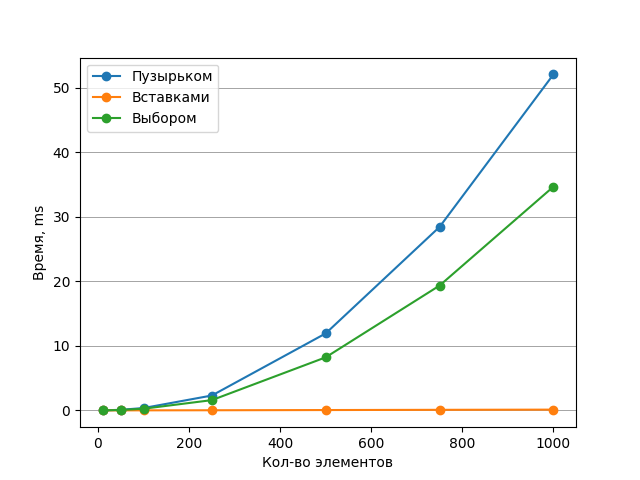
\includegraphics[scale=0.9]{imgs/forward.png}
	\caption{Зависимость времени работы алгоритмов от кол-ва элементов для отсортированного массива}
	\label{img:profiling-fwd}
\end{figure}
\newpage

Результаты для отсортированного в обратном порядке массива приведены в табл. \ref{tab:profiling-reverse} и на рис. \ref{tab:profiling-reverse}.
\begin{table}[!ht]
	\begin{center}
		\captionof{table}{Время выполнения алгоритмов (в мс) для отсортированного в обратном порядке массива}
		\begin{tabular}{|c|c|c|c|} 
			\hline
			Размер & Пузырьком & Вставками & Выбором \\  
			\hline
			10 & 0.0069 & 0.0042 & 0.0036 \\
			\hline
			50 & 0.1609 & 0.0872 & 0.0688 \\
			\hline
			100 & 0.6399 & 0.3416 & 0.2671 \\
			\hline
			250 & 4.0055 & 2.1369 & 1.6483 \\
			\hline
			500 & 19.0076 & 8.9443 & 8.6054 \\
			\hline
			750 & 46.0853 & 20.5732 & 20.2551 \\
			\hline
			1000 & 81.7425 & 36.9837 & 36.4731 \\
			\hline
		\end{tabular}
		\label{tab:profiling-reverse}
	\end{center}
\end{table}

\begin{figure}[!h]
	\centering
	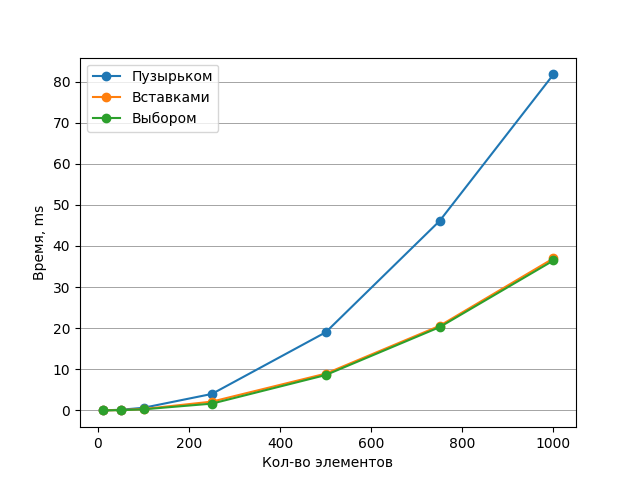
\includegraphics[scale=0.9]{imgs/reverse.png}
	\caption{Зависимость времени работы алгоритмов от кол-ва элементов при обратно отсортированном массиве}
	\label{img:profiling-reverse}
\end{figure}
\newpage

Результаты для неупорядоченного массива приведены в табл. \ref{tab:profiling-rand} и на рис. \ref{tab:profiling-rand}.
\begin{table}[!ht]
	\begin{center}
		\captionof{table}{Время выполнения алгоритмов (в мс) для неупорядоченного массива}
		\begin{tabular}{|c|c|c|c|} 
			\hline
			Размер & Пузырьком & Вставками & Выбором \\  
			\hline
			10 & 0.0058 & 0.0029 & 0.0036 \\
			\hline
			50 & 0.1308 & 0.0477 & 0.0687 \\
			\hline
			100 & 0.5152 & 0.1726 & 0.263 \\
			\hline
			250 & 3.2178 & 1.0676 & 1.6146 \\
			\hline
			500 & 15.8039 & 4.3968 & 8.3057 \\
			\hline
			750 & 37.7369 & 10.8403 & 19.4612 \\
			\hline
			1000 & 68.9718 & 19.3811 & 35.0158 \\
			\hline
		\end{tabular}
		\label{tab:profiling-rand}
	\end{center}
\end{table}

\begin{figure}[!h]
	\centering
	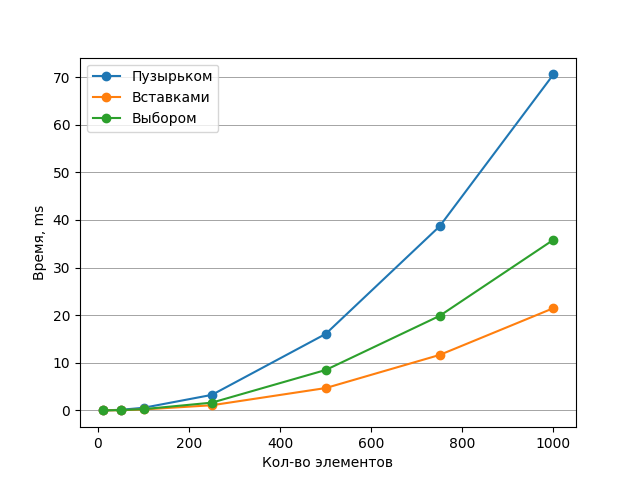
\includegraphics[scale=0.9]{imgs/random.png}
	\caption{Зависимость времени работы алгоритмов от кол-ва элементов при неупорядоченном массиве}
	\label{img:profiling-rand}
\end{figure}

\section{Вывод}

Алгоритмы сортировки пузырьком и выбором на отсортированных массивах работают медленнее, чем сортировка вставками.
Так уже при длине массива, равной 10 элементам, сортировка вставками быстрее сортировки выбором в три раза,
 а сортировки пузырьком - в четыре. С ростом размера массива преимущество только увеличивается: на массивах 
 с 1000 элементами сортировка вставками выполняется быстрее сортировки выбором в 300 раз,
а сортировки пузырьком в 430 раз.

На обратно отсортированных массивах сортировка вставками сравнима по быстродействию с сортировкой выбором.
При длине массива, равной 10 элементам, сортировка вставками медленнее сортировки выбором в 1.17 раз, при 500
элементах - 1.04, а при 1000 элементах всего лишь в 1.01 раз. При этом сортировка пузырьком медленнее остальных 
примерно в 2.2 раза.

Если рассматривать случай, более приближенный к реальности, когда массивы никак не упорядочены, то сортировка 
вставками снова оказывается быстрее остальных. Она быстрее сортировки выбором и пузырьком в 1.2 и 2 раза
соответственно при 10 элементах в массиве, в 1.9 и 3.6 раза - при 500 элементах, в 1.8 и 3.5 раза - при 1000 элементах.

Следовательно, можно сделать вывод, что сортировка вставками является наиболее эффективной сортировкой из рассмотренных,
а сортировка пузырьком, наоборот, наименее эффективной.